
\chapter{Special Matrices}
\subsection{Block matrices}
Stuff like Schur complements is interesting.
But can we say anything useful using tensor diagrams?

\subsection{The Discrete Fourier Transform Matrix}
I think FFT can be nicely described with diagrams

Let's start with the Hadamard matrix:
$H_n = \smat{1 & 1 \\ 1 & -1}^{\otimes n}$.
Hm. It's just a bunch of matrices below each other, kinda boring.

What about the FFT?
Does that require a bit more?





\subsection{Fast Kronecker Multiplication}

Say we want to compute $(A_1\otimes A_2\cdots A_n)x$,
where $A_i$ is a $a_i \times a_i$ matrix, and $x \in \R^{a_1 a_2 \cdots a_n}$.
If we first compute the Kronecker product, and then the matrix-vector multiplication, this would take $(a_1\cdots a_n)^2$ time.

Instead we can reshape $x$ into a $a_1 \times \cdots a_n$ tensor and 
perform the multiplication
\[
   \begin{tikzpicture}[baseline=-.25em]
      \node (A) at (1,.5) {$A_1$};
      \node (B) at (1,0) {$A_2$};
      \node (C) at (1,-0.4) {$\vdots$};
      \node (D) at (1,-1.1) {$A_n$};
      \node (x) at (2,0) {$X$};
      \draw (A) -- ++(-.6,0) node[midway, above, font=\tiny] {$a_1$};
      \draw (B) -- ++(-.6,0)node[midway, above, font=\tiny] {$a_2$};
      \draw ($(C.west)+(0,-.1)$) -- ++(-.4,0);
      \draw (D) -- ++(-.6,0) node[midway, below, font=\tiny] {$a_n$};
      \draw (A) -- (x) node[midway, above, font=\tiny] {$a_1$};
      \draw (B) -- (x);
      \draw ($(C.east)+(0,-.1)$) -- (x);
      \draw (D) -- (x) node[midway, below right, font=\tiny] {$a_n$};
   \end{tikzpicture}
%\quad\text{in time}
\]
by contracting the $a_i$ edges one by one.
This takes time
\[
a_1^2(a_2\cdots a_n)
+ a_2^2(a_1a_3\cdots a_n)
+ \dots
+ a_n^2(a_1\cdots a_{n-1})
= (a_1 + \dots + a_n)(a_1 \cdots a_n),
\]
which is the basis of many fast algorithm as we will see.

\subsubsection{Hadamard}

The Hadamard matrix is defined as
$
H_{2^n}
= H_2^{\otimes n}
= H_2 \otimes \dots\otimes H_2
$
where $H_2=\smat{1 & 1 \\ 1 & -1}$.
For example
\[
  \renewcommand*{\arraystretch}{1}
  H_4 =
  H_2 \otimes H_2
= \begin{bmatrix}
   H_{2}
   & H_{2}
   \\ H_{2}
   & -H_{2}
\end{bmatrix}
=  \begin{bmatrix}
    1 &  1 &  1 &  1\\
    1 & -1 &  1 & -1\\
    1 &  1 & -1 & -1\\
    1 & -1 & -1 &  1
  \end{bmatrix}.
\]
This gives a very simple tensor diagram representation as:
\[
H_{2^n} = 
   \begin{tikzpicture}[baseline=-.25em]
      \node[triangle, rotate=180] (F0) at (0,0) {};
      \node (A) at (1,.5) {$H_2$};
      \node[triangle] (F1) at (2,0) {};
      \node (B) at (1,0.1) {$\vdots$};
      \node (C) at (1,-.5) {$H_2$};
      \draw[double] (F0) -- ++(-.4,0);
      \draw[double] (F1) -- ++(.4,0);
      \draw (F0) -- (A) -- (F1);
      \draw (F0) -- (B) -- (F1);
      \draw (F0) -- (C) -- (F1);
   \end{tikzpicture}
   \,.
\]
The Fast Hadamard Transform (FHT) transform is usually described recursively by:
\[
   \renewcommand*{\arraystretch}{1.3}
H_{2^n} x
= \begin{bmatrix}
   H_{2^{n-1}} 
   & H_{2^{n-1}} 
   \\ H_{2^{n-1}} 
   & -H_{2^{n-1}} 
\end{bmatrix}
\begin{bmatrix}
    x^{(1)}
    \\
    x^{(2)}
\end{bmatrix}
,
\]
where $\smat{ x^{(1)} \\ x^{(2)} }$ is the first and second half of $x$.
Because of the redundancy in the matrix multiplication (it only depends on $H_{2^{n-1}}x^{(1)}$ and $H_{2^{n-1}} x^{(2)}$, the algorithm computes $H_N x$ in $O(N\log N)$ time.

Alternatively we could just use the general fact, as described above, where $a_i = 2$ for all $i$.
Then the ``fast Kronecker multiplication'' method takes time $(a_1 a_2\cdots a_n)(a_1+a_2+\cdots a_n) = 2 n \log_2 n$.


\subsubsection{Fourier}

% A more common matrix is the Discrete Fourier Matrix.
%\\
%\\
The Discrete Fourier Matrix is defined by $(F_N)_{i,j}=\omega^{ij}$,
where $\omega = e^{-2\pi i/N}$:
%We can write it out as
\[
   \renewcommand*{\arraystretch}{1}
F_N =
   \begin{bmatrix}
      1&1&1&1&\cdots &1 \\
      1&\omega&\omega^2&\omega^3&\cdots&\omega^{N-1} \\
      1&\omega^2&\omega^4&\omega^6&\cdots&\omega^{2(N-1)}\\ 1&\omega^3&\omega^6&\omega^9&\cdots&\omega^{3(N-1)}\\
      \vdots&\vdots&\vdots&\vdots&\ddots&\vdots\\
      1&\omega^{N-1}&\omega^{2(N-1)}&\omega^{3(N-1)}&\cdots&\omega^{(N-1)(N-1)}
   \end{bmatrix}
.
\]
\[
   =
   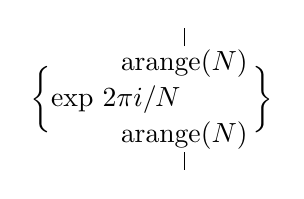
\begin{tikzpicture}[baseline=-.25em, y=1.3em, inner sep=1pt]
      \node at (0,0) {$\bigg\{\mathrm{exp} \,\, 2\pi i/N$};
      \node (a) at (1,1) {$\mathrm{arange}(N)$};
      \node (b) at (1,-1) {$\mathrm{arange}(N)$};
      \node at (2,0) {$\bigg\}$};
      \draw (a.north) -- ++(0, .5);
      \draw (b.south) -- ++(0, -.5);
   \end{tikzpicture}
\]
TODO: Show how the matrix can be written with the function notation.

The Good-Thomas Fast Fourier Transformer (FFT) uses a decomposition based on the Chinese Remainder Theorem:
\[
F_{N} = 
   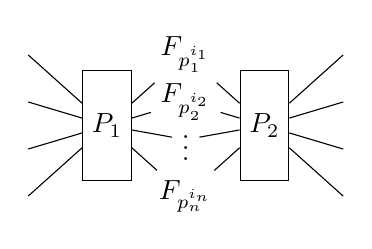
\begin{tikzpicture}[baseline=-1em, y=1.7em]
      \node[rectangle, draw, minimum height=4em] (P1) at (0,-.5) {$P_1$};
      \node (A) at (1,1) {$F_{p_1^{i_1}}$};
      \node[rectangle, draw, minimum height=4em] (P2) at (2,-.5) {$P_2$};
      \node (B) at (1,0) {$F_{p_2^{i_2}}$};
      \node (C) at (1,-.8) {$\vdots$};
      \node (D) at (1,-2) {$F_{p_n^{i_n}}$};
      \draw (-1,1) -- (P1) -- (A) -- (P2) -- (3, 1);
      \draw (-1,0) -- (P1) -- (B) -- (P2) -- (3, 0);
      \draw (-1,-1) -- (P1) -- (C) -- (P2) -- (3, -1);
      \draw (-1,-2) -- (P1) -- (D) -- (P2) -- (3, -2);
   \end{tikzpicture}
   \,,
\]
where $N = p_1^{i_1} p_2^{i_2} \cdots p_n^{i_n}$ is the prime factorisation of $N$, and $P_1$ and $P_2$ are some permutation matrices.

Using fast Kronecker multiplication, the algorithm this takes $(p_1^{i_1}+\dots+p_n^{i_n}) N$ time.
By padding $x$ with zeros, we can increase $N$ by a constant factor to get a string of $n=O(\log(N)/\log\log(N))$ primes, the sum of which is $\sim n^2/\log n = O(\log(N)^2)$.
The complete algorithm thus takes time $O(N \log(N)^2)$.
Next we will see how to reduce this to $O(N\log N)$.

The classical Cooley-Tukey FFT algorithm uses a recursion:
\[
   \renewcommand*{\arraystretch}{1.3}
F_N =
\begin{bmatrix}
I & I \\
I & -I
\end{bmatrix}
\begin{bmatrix}
I & 0 \\
0 & D_{N/2}
\end{bmatrix}
\begin{bmatrix}
F_{N/2} & 0 \\
0 & F_{N/2}
\end{bmatrix}
\begin{bmatrix}
\text{even-odd} \\
\text{permutation}
\end{bmatrix}
,
\]
where $D_N = [1, w^N, w^{2N}, \dots]$.
The even-odd permutation moves all the even values to the start.
If we reshape $I_{2^n}$ as $I_2\otimes\dots\otimes I_2$, this permutation is just
$
P_N = 
\begin{tikzpicture}[baseline=.5em, x=1em, y=.5em]
    \draw (0,0) -- (1, 1);
    \draw (0,1) -- (1, 2);
    \draw (0,2) -- (1, 3);
    \draw (0,3) -- (1, 0);
\end{tikzpicture}
$,
or in pytorch: \texttt{x.permute([3,0,1,2])}.
Also note that
$\smat{I&I\\I&-I} = H_2 \otimes I$ and $\smat{F_{N/2} & 0\\0&F_{N/2}}=I_2 \otimes F_{N/2}$.
So we can write in tensor diagram notation:
\begin{align*}
F_N =
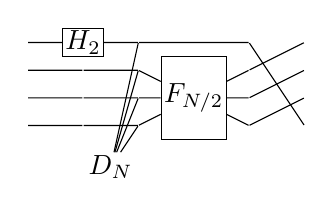
\begin{tikzpicture}[baseline=-2em, x=2em, y=1em, inner sep=1pt]
    \node[rectangle,draw] (H) at (0,0) {$H_2$};
    \node[inner sep=0pt, minimum size=0pt] (l1) at (0,-1) {};
    \node[inner sep=0pt, minimum size=0pt] (l2) at (0,-2) {};
    \node[inner sep=0pt, minimum size=0pt] (l3) at (0,-3) {};
    \node[inner sep=0pt, minimum size=0pt] (L0) at (-1,0) {};
    \node[inner sep=0pt, minimum size=0pt] (L1) at (-1,-1) {};
    \node[inner sep=0pt, minimum size=0pt] (L2) at (-1,-2) {};
    \node[inner sep=0pt, minimum size=0pt] (L3) at (-1,-3) {};
    \node[inner sep=0pt, minimum size=0pt] (b0) at (1,0) {$\sbullet$};
    \node[inner sep=0pt, minimum size=0pt] (b1) at (1,-1) {$\sbullet$};
    \node[inner sep=0pt, minimum size=0pt] (b2) at (1,-2) {$\sbullet$};
    \node[inner sep=0pt, minimum size=0pt] (b3) at (1,-3) {$\sbullet$};
    \node (D) at (.5,-4.5) {$D_N$};
    \node[rectangle,draw,minimum height=3em] (F) at (2,-2) {$F_{N/2}$};
    \node[inner sep=0pt, minimum size=0pt] (r0) at (4,0) {};
    \node[inner sep=0pt, minimum size=0pt] (r1) at (4,-1) {};
    \node[inner sep=0pt, minimum size=0pt] (r2) at (4,-2) {};
    \node[inner sep=0pt, minimum size=0pt] (r3) at (4,-3) {};
    \node[inner sep=0pt, minimum size=0pt] (s0) at (3,0) {};
    \node[inner sep=0pt, minimum size=0pt] (s1) at (3,-1) {};
    \node[inner sep=0pt, minimum size=0pt] (s2) at (3,-2) {};
    \node[inner sep=0pt, minimum size=0pt] (s3) at (3,-3) {};
    \draw (b0) -- (D);
    \draw (b1) -- (D);
    \draw (b2) -- (D);
    \draw (b3) -- (D);
    \draw (L0) -- (H) -- (b0) -- (s0) -- (r3);
    \draw (L1) -- (l1) -- (b1) -- (F) -- (s1) -- (r0);
    \draw (L2) -- (l2) -- (b2) -- (F) -- (s2) -- (r1);
    \draw (L3) -- (l3) -- (b3) -- (F) -- (s3) -- (r2);
\end{tikzpicture}
&=
\begin{tikzpicture}[baseline=-2em, x=2em, y=1em, inner sep=1pt]
    % Draw H nodes and connections
    \foreach \i in {0,...,3} {
        \node[rectangle,draw] (H\i) at (2*\i,-\i) {$H_2$};
        \node[inner sep=0pt, minimum size=0pt] (l\i) at (0,-\i) {};
        \node[inner sep=0pt, minimum size=0pt] (L\i) at (-1,-\i) {};
        \node[inner sep=0pt, minimum size=0pt] (s\i) at (7,-\i) {};
        \node[inner sep=0pt, minimum size=0pt] (r\i) at (8,-\i) {};
    }
    % Draw D nodes and connections to sbullets
    \foreach \i in {0, 1, 2} {
        \node (D\i) at (0.5+\i*2,-4.5) {$D_{N/2^\i}$};
        \foreach \k in {\i,...,3} {
            \node[inner sep=0pt, minimum size=0pt] (b\i\k) at (1+\i*2,-\k) {$\sbullet$};
            \draw (b\i\k) -- (D\i);
        }
    }
    \draw (L0) -- (H0) -- (b0) -- (s0) -- (r3);
    \draw (L1) -- (l1) -- (b1) -- (H1) -- (b11) -- (s1) -- (r2);
    \draw (L2) -- (l2) -- (b2) -- (b12) -- (H2) -- (b22) -- (s2) -- (r1);
    \draw (L3) -- (l3) -- (b3) -- (b13) -- (b23) -- (H3) -- (s3) -- (r0);
\end{tikzpicture}
%\\&=
%\begin{tikzpicture}[baseline=-2em, x=2em, y=1em, inner sep=1pt]
%    % Draw H nodes and connections
%    \foreach \i in {0,...,3} {
%        \node[rectangle,draw] (H\i) at (2*\i,-3+\i) {$H_2$};
%        \node[inner sep=0pt, minimum size=0pt] (l\i) at (0,-\i) {};
%        \node[inner sep=0pt, minimum size=0pt] (L\i) at (-1,-\i) {};
%        \node[inner sep=0pt, minimum size=0pt] (s\i) at (7,-\i) {};
%        \node[inner sep=0pt, minimum size=0pt] (r\i) at (-2,-\i) {};
%    }
%    % Draw D nodes and connections to sbullets
%    \foreach \i in {0, 1, 2} {
%        \node (D\i) at (0.5+\i*2,-4.5) {$D_{N/2^\i}$};
%        \foreach \k in {\i,...,3} {
%            \node[inner sep=0pt, minimum size=0pt] (b\i\k) at (1+\i*2,-\k) {$\sbullet$};
%            \draw (b\i\k) -- (D\i);
%        }
%    }
%    \draw (r3) -- (L0) -- (H3) -- (b0) -- (s0);
%    \draw (r2) -- (L1) -- (l1) -- (b1) -- (H2) -- (b11) -- (s1);
%    \draw (r1) -- (L2) -- (l2) -- (b2) -- (H1) -- (b12) -- (b22) -- (s2);
%    \draw (r0) -- (L3) -- (H0) -- (l3) -- (b3) -- (b13) -- (b23) -- (s3);
%\end{tikzpicture}
.
\end{align*}
Since one can multiply with the permutation and diagonal matrices in linear time, the $O(n\log n)$ time complexity follows from the same argument as for Hadamard.

Note there are a bunch of symmetries, such as by transposing (horizontal flip), since the matrix is symmetric.
Or by pushing the permutation to the left side.

We don't have to split the matrix in half, we can also split it in thirds, fourths, etc.
With this generalized Cooley-Tukey algorithm, we get the following diagram:
\[
   F_N =
\begin{tikzpicture}[baseline=-2em, x=2em, y=1em, inner sep=1pt]
    % Draw H nodes and connections
    \foreach \i in {0,...,3} {
        \node[rectangle,draw] (H\i) at (2*\i,-\i) {$F_{n_\i}$};
        \node[inner sep=0pt, minimum size=0pt] (L\i) at (-1,-\i) {};
        \node[inner sep=0pt, minimum size=0pt] (s\i) at (7,-\i) {};
        \node[inner sep=0pt, minimum size=0pt] (r\i) at (8,-\i) {};
    }
    % Draw D nodes and connections to sbullets
    \node (D0) at (0.5+0*2,-4.5) {$\scriptstyle F^{(n_0, n_1n_2n_3)}$};
    \node (D1) at (0.5+2.2,-4.5) {$\scriptstyle F^{(n_1, n_2n_3)}$};
    \node (D2) at (0.5+2*2,-4.5) {$\scriptstyle F^{(n_2, n_3)}$};
    \foreach \i in {0, 1, 2} {
        \foreach \k in {\i,...,3} {
            \node[inner sep=0pt, minimum size=0pt] (b\i\k) at (1+\i*2,-\k) {$\sbullet$};
            \draw (b\i\k) -- (D\i);
        }
    }
    \draw (L0) -- (H0) -- (b0) -- (s0) -- (r3);
    \draw (L1) -- (b1) -- (H1) -- (b11) -- (s1) -- (r2);
    \draw (L2) -- (b2) -- (b12) -- (H2) -- (b22) -- (s2) -- (r1);
    \draw (L3) -- (b3) -- (b13) -- (b23) -- (H3) -- (s3) -- (r0);
\end{tikzpicture}
,
\]
where $n_0n_1n_2n_3 = N$.
Here we replaced the $D_N$ matrix with the ``generalized'' Fourier matrix $F^{(a,b)}$ matrix, which is defined as $F^{(a,b)}_{j,k} = e^{-2\pi i j k/(ab)}$, and we reshaped as necessary.
In the simple case of where we split in just two parts of roughly $n_1=n_2=\sqrt{N}$, this is also called ``Four step FFT'' or Bailey's FFT algorithm.

We can use the property $F_{a,bc} = F_{a,b} \bullet F_{a,c}^{1/b}$ to simplify the diagram further:
\[
   F_N =
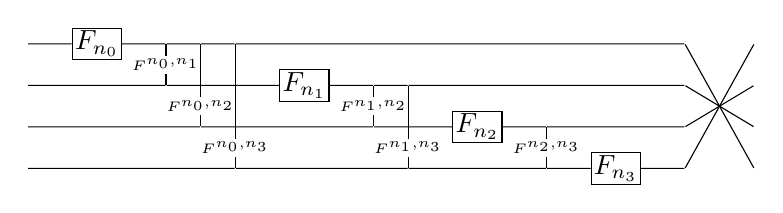
\begin{tikzpicture}[baseline=-2em, x=2.5em, y=1.5em, inner sep=1pt]
    % Draw H nodes and connections
    \foreach \i in {0,...,3} {
        \node[rectangle,draw] (H\i) at (3.25*\i-\i*\i/4,-\i) {$F_{n_\i}$};
        \node[inner sep=0pt, minimum size=0pt] (L\i) at (-1,-\i) {};
        \node[inner sep=0pt, minimum size=0pt] (s\i) at (8.5,-\i) {};
        \node[inner sep=0pt, minimum size=0pt] (r\i) at (9.5,-\i) {};
    }
    % Draw D nodes and connections to sbullets
    \foreach \i in {0, 1, 2} {
        \pgfmathtruncatemacro{\j}{\i+1}
        \foreach \k in {\j,...,3} {
            \node[inner sep=0pt, minimum size=0pt] (b\i\k) at (1/2+2.75*\i-\i*\i/4+\k/2,-\i) {$\sbullet$};
            \node[inner sep=0pt, minimum size=0pt] (c\i\k) at (1/2+2.75*\i-\i*\i/4+\k/2,-\k) {$\sbullet$};
        }
    }
    \node (D00) at (1,-.5) {$\scriptscriptstyle F^{n_0, n_1}$};
    \node (D01) at (1.5,-1.5) {$\scriptscriptstyle F^{n_0, n_2}$};
    \node (D02) at (2,-2.5) {$\scriptscriptstyle F^{n_0, n_3}$};
    \draw (b01) -- (D00) -- (c01);
    \draw (b02) -- (D01) -- (c02);
    \draw (b03) -- (D02) -- (c03);
    \node (D10) at (4,-1.5) {$\scriptscriptstyle F^{n_1, n_2}$};
    \node (D11) at (4.5,-2.5) {$\scriptscriptstyle F^{n_1, n_3}$};
    \draw (b12) -- (D10) -- (c12);
    \draw (b13) -- (D11) -- (c13);
    \node (D20) at (6.5,-2.5) {$\scriptscriptstyle F^{n_2, n_3}$};
    \draw (b23) -- (D20) -- (c23);
    % Horizontal connections
    \draw (L0) -- (H0) -- (b01) -- (b02) -- (b03) -- (s0) -- (r3);
    \draw (L1) -- (c01) -- (H1) -- (b12) -- (b13) -- (s1) -- (r2);
    \draw (L2) -- (c02) -- (c12) -- (H2) -- (b23) -- (s2) -- (r1);
    \draw (L3) -- (c03) -- (c13) -- (c23) -- (H3) -- (s3) -- (r0);
\end{tikzpicture}
.
\]
% This algorithm is actually slower (n (log n)^2), because the pair-wise D matrices are not actually faster.
In the simple case where we split in $2$ every time, this is also called the ``Quantum FFT'' algorithm.

We hid some stuff above, namely that the matrices should be divided by different $N$s.


Note that this figure may look different from some FFT diagrams you have seen.
These typically look like this:
\[
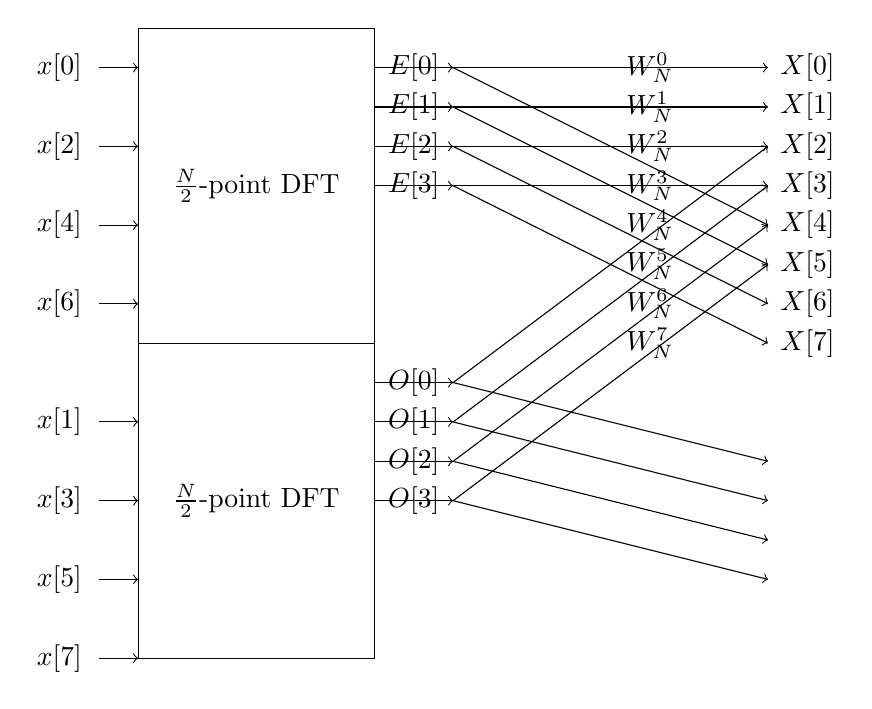
\begin{tikzpicture}
  % Draw N/2-point DFT blocks
  \draw (0, 1) rectangle (3, 5) node[midway] {$\frac{N}{2}$-point DFT};
  \draw (0, -3) rectangle (3, 1) node[midway] {$\frac{N}{2}$-point DFT};

  % Input nodes
  \foreach \i in {0,2,4,6} {
    \node at (-1, 4.5 - \i*0.5) {$x[\i]$};
    \draw[->] (-0.5, 4.5 - \i*0.5) -- (0, 4.5 - \i*0.5);
  }
  
  \foreach \i in {1,3,5,7} {
    \node at (-1, 4.5 - \i*0.5 - 4) {$x[\i]$};
    \draw[->] (-0.5, 4.5 - \i*0.5 - 4) -- (0, 4.5 - \i*0.5 - 4);
  }

  % Intermediate outputs E and O
  \foreach \i in {0,1,2,3} {
    \node at (3.5, 4.5 - \i*0.5) {$E[\i]$};
    \draw[->] (3, 4.5 - \i*0.5) -- (4, 4.5 - \i*0.5);
  }
  
  \foreach \i in {0,1,2,3} {
    \node at (3.5, 4.5 - \i*0.5 - 4) {$O[\i]$};
    \draw[->] (3, 4.5 - \i*0.5 - 4) -- (4, 4.5 - \i*0.5 - 4);
  }

  % Output nodes X
  \foreach \i in {0,...,7} {
    \node at (8.5, 4.5 - \i*0.5) {$X[\i]$};
  }
  
  % W_N terms
  \foreach \i in {0,...,7} {
    \node at (6.5, 4.5 - \i*0.5) {$W_N^{\i}$};
  }

  % Connections from E and O to X
  \foreach \i in {0,...,3} {
    \draw[->] (4, 4.5 - \i*0.5) -- (8, 4.5 - \i*0.5);
    \draw[->] (4, 4.5 - \i*0.5) -- (8, 4.5 - \i*0.5 - 2);
  }
  
  \foreach \i in {0,...,3} {
    \draw[->] (4, 4.5 - \i*0.5 - 4) -- (8, 4.5 - \i*0.5 - 1);
    \draw[->] (4, 4.5 - \i*0.5 - 4) -- (8, 4.5 - \i*0.5 - 5);
  }
\end{tikzpicture}
\]
and have $2^n$ rows.
The tensor diagram only has $n$ rows (or $\log_2 N$).

\subsubsection{Multi-dimensional Fourier Transform}
This is just taking the Fourier transform along each axis.

\newpage


\subsection{Hermitian Matrices and skew-Hermitian}
Complex. Skip
\subsection{Idempotent Matrices}
Skip
\subsection{Orthogonal matrices}
Skip
\subsection{Positive Definite and Semi-definite Matrices}
Skip
\subsection{Singleentry Matrix, The}
Describes the matrix $J$.
All of this is trivial with diagrams.
\subsection{Symmetric, Skew-symmetric/Antisymmetric}

Could introduce Penrose's symmetric tensors here?

\subsection{Toeplitz Matrices}
Could talk about the convolution tensor here...
\subsection{Units, Permutation and Shift}
Not that interesting...
\subsection{Vandermonde Matrices}
Does this have a nice description?
Not a lot of properties are given in the Cookbook.


